\documentclass[11pt]{article}
\usepackage[margin=1in]{geometry}
\usepackage{graphicx,booktabs,amsmath,amssymb,xcolor,caption,hyperref,enumitem}
\usepackage[numbers,sort&compress]{natbib}
\hypersetup{colorlinks=true,linkcolor=blue,citecolor=blue,urlcolor=blue}
\graphicspath{{figures/}}
\captionsetup{font=small,labelfont=bf}
\title{\textbf{Certainty Is Outsourced Trust:\\ Mechanism-Grounded, Black-Box Fuzzing of Multi-Agent LLM Systems}}
\author{(draft for review)}
\date{}

\begin{document}
\maketitle

\begin{abstract}
Multi-agent LLM systems (MAS) increasingly authorize consequential tool actions behind a safety assumption: an
upstream auditor agent will catch a malicious request before a decider acts. A recent measurement study---the
\emph{capability paradox}---unsettles this: a \emph{more} capable auditor can make the system \emph{more}
hijackable, mediated by the auditor's linguistic \emph{certainty}. We turn that mediator into a fuzzing fitness.
\textsc{MASFuzzer} is a black-box, coverage-guided fuzzer: an attacker LLM rewrites the entry request to climb
the auditor's output certainty while preserving a coherent incident narrative. In the canonical Manager--Worker
topology, certainty-steering roughly \emph{doubles} attack success over a fair same-LLM baseline (paired
difference $+0.176$, cluster-bootstrap 95\% CI $[+0.09,+0.26]$ over 3 seeds, $n{=}216$/arm) with coherence held,
and shows a certainty$\to$hijack dose-response that survives a pseudoreplication-corrected (cluster-robust) test
($p{<}.01$) and replicates across three independent campaigns ($\rho\approx0.25$ each). Sweeping five architectures, we find the
advantage is \emph{not} a universal rule but is governed by a single mechanism. Each topology is hijacked through
whether the upstream content the decider trusts \emph{endorses} the action---certainty for an auditor,
endorsement-transfer for a handoff swarm, vote-balance for a broadcast group-chat---and the effect size scales
with how much the decider \emph{outsources} safety judgment to a separable upstream verdict. We confirm this
causally: inserting an auditor into an otherwise-robust swarm raises ASR $0.36\to0.54$ and makes certainty a
steerable causal lever ($\rho{=}0.26$, $p{=}.008$), even though the executor still judges. This resolves why the
capability paradox's \emph{judging} manager is hijacked at all---it sits at the full-outsourcing end of the
continuum.
\end{abstract}

\section{Introduction}
LLM multi-agent systems now triage incidents, write to databases, and call infrastructure tools with limited
human oversight. A central safety assumption is that an upstream auditor or reviewer agent catches a malicious or
mistaken request before a decider acts on it. The capability paradox~\cite{liu2026capabilityparadox} unsettles
this: a \emph{more} capable auditor can make the system \emph{more} hijackable, because a confidently-worded
``safe'' verdict is precisely what persuades the decider to comply---a failure mode they term \emph{semantic
hijacking}, mediated by the auditor's linguistic certainty.

Turning this observation into a systematic attack generator is unaddressed. White-box MAS fuzzers
(\textsc{FLARE}~\cite{flare2026}) need agent source and target functional reliability, not security; single-agent
prompt-injection fuzzers (\textsc{AgentVigil}~\cite{agentvigil2025}) do not model the multi-agent decision path;
and quality-diversity red-teaming~\cite{rainbow2024,qdrt2025,curiosity2024} searches input-side descriptors
against a single model. None steers by the causal mediator of the failure, and none asks how the right attack
depends on the MAS architecture.

We make the mediator the fuzzing fitness. \textsc{MASFuzzer} is black-box---it observes only agents' text---and an
attacker LLM rewrites the request to raise the auditor's output certainty while preserving a coherent incident
narrative, hill-climbing this continuous, causally-grounded signal. We then ask where across architectures the
lever pays off, and find a single unifying mechanism.

\noindent\textbf{Contributions.}
\begin{enumerate}[leftmargin=1.4em,itemsep=1pt]
\item We turn the capability-paradox mediator into a fuzzing fitness and confirm, \emph{in the attack loop}, a
certainty$\to$hijack dose-response that is robust to pseudoreplication (cluster-robust $p{<}.01$; consistent
across three independent campaigns).
\item A black-box, mechanism-grounded LLM-mutation fuzzer whose certainty-steering roughly doubles ASR over a
fair same-LLM baseline ($0.45$ vs $0.27$) with coherence held.
\item From $500$ payloads $\times\,14$ manager models we mine and \emph{adversarially verify} the framings that
make attacks succeed, and show coarse categories and input-text certainty do \emph{not} predict success.
\item A mechanism for \emph{which} signal hijacks \emph{which} architecture: a single endorsement-transfer law
modulated by judgment-\emph{outsourcing}, confirmed causally, which resolves the capability-paradox puzzle and
tells a defender exactly which topology to harden.
\end{enumerate}

\section{Threat Model and Problem}
A MAS is an ordered set of agents $A_1,\dots,A_n$, each a fixed (model, system-prompt) pair connected by a
topology $\tau$. Given a request $x$, the system produces a trace $T_\tau(x)$ and a final decision $d$. A
validated oracle $O(d)\in\{0,\dots,4\}$ grades it; a \emph{hijack} is $O(d)\ge 2$. The attacker submits only the
natural-language request at the entry point, with no access to weights, logits, system prompts, intermediate
traces, or tool feedback---the realistic setting for a third party interacting with a deployed agentic service.
The objective is to maximize the hijack rate under a query budget $B$.

\section{Method}
\label{sec:method}
\textbf{Certainty as a climbable fitness.} For the auditor (or first-agent) output $o$ we score linguistic
certainty $c(o)$ as the assertive-minus-hedging term density using the exact lexicon with which the mother
paper's mediation was measured. Certainty is a \emph{continuous, climbable} scalar; behavioral-diversity
descriptors, by contrast, saturate after a handful of samples and tie a random baseline.

\textbf{Certainty-guided LLM mutation.} An attacker LLM rewrites the parent request to maximize $c$ while keeping
one coherent incident narrative and preserving the dangerous action (few-shot on high-certainty exemplars). A
$\mu{+}\lambda$ hill-climb breeds the top-$k$ elites by $c$. The decisive baseline is the \emph{same} LLM
rewriting with no objective (\textsc{neutral}), isolating steering from LLM rewriting per se; we also compare to
\textsc{concat}, a hand-coded random-operator baseline.

\textbf{Success-condition mining.} Using $500$ payloads $\times\,14$ real manager models from existing
oracle-graded logs (zero new queries), a multi-agent pipeline contrasts the cross-manager success extremes,
labels the corpus, and adversarially verifies each candidate framing against strategy/tool-matched controls.

\section{Experiments and Results}
\textbf{Setup.} We evaluate on \texttt{paradox\_dataset\_500} (500 SRE incident-response prompt-injection
payloads). Weak agents are Llama-3.2-3B, the attacker/mutator and strong decider are DeepSeek-V3, and the oracle
is the capability-paradox-validated GPT-4o-mini judge ($\kappa\ge0.87$), under a strict decision SOP (the regime
in which ASR is intermediate and guidance can discriminate). Primary metric: ASR; secondary: deep-capture
(grade$\ge3$), coherence (judge plausibility), dose-response. \emph{Statistics.} We treat the random seed as the
experimental unit (3 seeds, $72$ candidates/arm/seed); the headline uses a cluster bootstrap (resampling
candidates within each (seed,arm)), the dose-response a cluster-robust GEE plus per-seed correlations (to avoid
pseudoreplication), and all mechanism $p$-values are Holm--Bonferroni corrected. We flag $n{=}3$ seeds as a
limitation and recommend $5$ for camera-ready.

\textbf{Certainty is a climbable fitness.} ASR climbs across worker-certainty bins from $0.20$ to $0.52$
(Fig.~\ref{fig:dose}), with one honest attenuation at the extreme bin (maximally assertive reports begin to read
as implausible). A naive pooled correlation ($\rho{=}0.25$, $p{=}5{\times}10^{-11}$) over-states significance,
since hill-climb candidates are autocorrelated; the effect nonetheless survives a cluster-robust GEE
($p{=}.010$) and replicates across all three independent campaigns ($\rho{=}0.25,0.27,0.26$; each $p{<}10^{-3}$).
Crucially, the certainty of the \emph{input payload} does \emph{not} predict cross-manager success
($\rho\approx0.05$, n.s.)---the lever is the auditor's \emph{output}.

\textbf{Certainty-steering beats fair baselines.} In the Manager--Worker topology at $n{=}216$/arm
(Fig.~\ref{fig:tab2}), certainty-steering reaches ASR $0.45$ vs $0.27$ (\textsc{neutral}) and $0.37$
(\textsc{concat}); the paired certainty$-$neutral difference is $+0.176$ with a cluster-bootstrap 95\% CI of
$[+0.09,+0.26]$ (excludes $0$; paired-$t$ $p{=}.025$ over 3 seeds), and coherence is held ($0.94$ vs $0.88$). The
synthesized attacks read as realistic incident reports.

\textbf{Cross-model robustness.} The mechanism is not specific to one model pair. Replacing the weak agent with
a second family (Qwen-2.5-7B), the certainty$\to$hijack dose-response holds at the supervisor edge
($\rho{=}0.36$--$0.47$, $p{<}10^{-3}$) and the swarm+auditor causal anchor remains significant
($\rho(\text{auditor cert},\text{grade}){=}0.31$, $p{=}.002$). The \emph{more capable} Qwen worker is markedly
\emph{more} hijackable overall (certainty-arm ASR ceilings at $0.98$--$1.00$ vs $\approx0.45$ for Llama-3.2-3B,
and a strong DeepSeek decider does not lower it)---itself a prediction of the capability paradox (more capable
auditor $\to$ more confident $\to$ more hijackable). The mechanism thus translates across the model axis, while
its absolute strength scales with worker capability, as the paradox predicts.

\textbf{What makes attacks succeed.} Per-payload cross-manager success ranges $0.00$--$0.85$. Coarse strategy/
tool categories barely move ASR ($15$--$20\%$) and saturated tactics (urgency, assertiveness) fail adversarial
verification. The verified conditions are framings of \emph{how the destruction is presented}: a live
external-attacker reframe ($42$--$46\%$ of high-success vs $8\%$ of blocked payloads), a first-person commander
voice with forensic certainty ($67\%$ vs $27\%$), a euphemized action verb ($80\%$ vs $8\%$), a named recovery
source on an irreplaceable target, an omitted loss-disclosure, and third-party/compliance stakes.

\textbf{Where does it generalize \emph{as an attack}?} Sweeping five architectures over four configurations
(Fig.~\ref{fig:tab5}), exactly one cell yields a \emph{stable, high-effect} certainty attack across all
configurations and both scales: the supervisor (auditor$\to$manager) topology ($0.52\pm.06$). Every other
topology is unstable at the ASR level (the single fused agent flips with scale; pipeline is a wash; group-chat
and swarm are high-variance). We are careful to separate two questions: whether \emph{steering a signal is a
strong, reliable attack} (answered here---only at the supervisor edge), and whether \emph{a signal is the causal
mechanism of hijacking} in a topology (Sec.~\ref{sec:mech}). A lever can be a genuine mechanism even where
steering it is not yet a high-variance-free attack; the next section establishes the mechanism and anchors it
with two causal experiments.

\section{The Hijack Mechanism: an Outsourcing Continuum}
\label{sec:mech}
Why does certainty dominate the supervisor but not other topologies? We probed each architecture for its own
hijack lever, classifying every upstream agent's stance toward the action with a judge and correlating
architecture-specific features with the hijack grade (Table~\ref{tab:levers}).

\begin{table}[t]\centering\small
\caption{Each architecture's hijack lever (Spearman correlation with the hijack grade). All are the same
underlying quantity---whether the upstream content the decider trusts \emph{endorses} the action---in
topology-native form. $p$-values are Holm--Bonferroni corrected over the seven lever/causal tests of Sec.~5;
${}^{\dagger}$ marks cells that are Holm-significant but only \emph{suggestive} under the stricter Bonferroni.}
\label{tab:levers}
\begin{tabular}{@{}llccc@{}}
\toprule
Architecture & Lever (form of endorsement) & $\rho$ & raw $p$ & Holm $p$ \\
\midrule
supervisor & auditor's confident ``safe'' verdict (certainty) & $+0.49$ & $.0003$ & $.002$ \\
swarm & triage/specialist endorsement (handoff) & $+0.45$ & $.001$ & $.006$ \\
group-chat & endorsement balance of the debate (vote) & $+0.26$ & $.029$ & $.029^{\dagger}$ \\
pipeline & the plan's certainty/stance (survives re-plan) & $+0.36$ & $.011$ & $.025^{\dagger}$ \\
single & no separate endorser to exploit & --- & --- & --- \\
\bottomrule
\end{tabular}
\end{table}

The lever is the \emph{same underlying quantity}---whether the upstream content the decider trusts endorses the
action---expressed in each topology's native form (Fig.~\ref{fig:endorse}). Certainty is simply the form
endorsement takes at an auditor edge. A multivariate analysis rejects a \emph{combinatorial} explanation: a
single feature wins or ties in five of six architectures, so the cross-architecture variation is ``a different
lever per architecture,'' not a feature combination within one space.

\emph{Scope and evidence strength.} Table~\ref{tab:levers} is a \emph{correlational} mechanism map: every lever
is Holm-significant, though group-chat and pipeline are only suggestive under the stricter Bonferroni and we
mark them so. The continuum claim does not rest on these correlations alone---it is anchored by two
\emph{causal} steering experiments (supervisor and swarm+auditor, below). We therefore present the continuum as
a mechanism with two causal anchors plus a Holm-significant correlational map, not as a proven universal law;
strengthening the suggestive cells to causal status is future work.

\textbf{The capability-paradox puzzle, and its causal resolution.} If the lever is endorsement, why is the
capability paradox's \emph{judging} manager hijacked by certainty, while our swarm---whose executor also
judges---resists it? Because the decisive condition is not whether the decider judges (it always does) but
whether it \emph{outsources} its safety judgment to a separable upstream verdict it anchors on. We test this:
inserting a separable safety auditor into the swarm (triage$\to$auditor$\to$executor) raises ASR $0.36\to0.54$
and makes certainty a \emph{steerable causal} lever---certainty-steering the auditor lifts ASR $0.46\to0.52$ with
$\rho(\text{auditor certainty},\text{grade}){=}0.26$, $p{=}.008$---even though the executor still judges, whereas
plain-swarm certainty is null ($\rho\approx0.08$).

The certainty/endorsement effect size therefore scales with the degree of judgment-outsourcing
(Fig.~\ref{fig:outsourcing}): \emph{full} outsourcing (supervisor / the capability paradox) $\to$ certainty is a
strong, steerable attack ($0.27\to0.45$, ${\sim}2\times$); \emph{partial} (swarm+auditor) $\to$ moderate but
causal ($0.46\to0.52$, Holm $p{=}.025$); \emph{none} (fused single agent, or a swarm of routers) $\to$ null. The
two endpoints of this continuum are exactly the two cells with causal steering evidence, which is what licenses
reading it as one mechanism modulated by how much the decider anchors on a separable upstream verdict---rather
than as the per-architecture coincidences the correlational map alone would permit. This is why the capability
paradox's manager, which fully defers to the worker's verdict, is so reliably hijacked.

\section{Defense}
The attack exploits one trust relationship: deciders defer to confidently-worded upstream verdicts. Defenses
belong at that relationship, not at agent capability (raising the auditor's capability is what creates the
paradox). The supervisor (Manager--Worker) topology is where certainty-steering most reliably succeeds and
should receive the strongest decider-side certainty-skepticism (e.g.\ down-weighting an upstream verdict by its
assertiveness, or requiring the decider to re-derive the safety judgment rather than anchor on it). The
outsourcing continuum gives a design rule: the more a decider anchors on a separable upstream verdict, the more
it must discount that verdict's confidence.

\section{Related Work}
The closest line fuzzes LLM agents. \textsc{FLARE}~\cite{flare2026} brings coverage-guided fuzzing to MAS but is
white-box (reads agent source) and reliability-oriented; \textsc{ChainFuzzer}~\cite{chainfuzzer2026} targets
workflow-level multi-tool dataflow bugs; \textsc{AgentVigil}~\cite{agentvigil2025} is black-box and
security-oriented but single-agent and offers no account of \emph{why} an injection succeeds. Quality-diversity
red-teaming~\cite{rainbow2024,qdrt2025,autoqd2025,curiosity2024} and \textsc{T-MAP}~\cite{tmap2026} search
input/behavior/trajectory descriptors, mostly against a single model, rather than a causal mediator inside a MAS.
\textsc{MAST}~\cite{mast2025} taxonomizes MAS failures descriptively; \textsc{AiTM}~\cite{aitm2025} manipulates
the inter-agent channel (we assume entry-point access only). The capability
paradox~\cite{liu2026capabilityparadox} establishes the phenomenon we weaponize and measures the certainty
mediator (robust worker-only, weaker full-MAS); it is a measurement study, not an attack generator. To our
knowledge this is the first black-box, mechanism-grounded prompt-injection attack synthesizer for LLM
multi-agent systems, with a unified, causally-tested account of which signal hijacks which architecture.

\section{Limitations and Ethics}
\textbf{Limitations.} Our regime is a strict SOP with a weak auditor, chosen because it yields an intermediate
ASR where guidance can discriminate; a permissive SOP saturates ASR. We abstract five topologies homogeneously
rather than instrumenting full frameworks. We replicate the mechanism on a second weak-agent family
(Qwen-2.5-7B; both anchors significant) but a broader model sweep and real-framework deployments remain. On the
more capable Qwen worker the certainty arm ceilings, so its headline gap is compressed (the dose-response and the
causal anchor, however, both replicate). The cross-architecture causal effects
(swarm, swarm+auditor) are significant but modest; the headline effect is at the supervisor edge. Some
mixed cells retain wide error bars at 3--4 seeds.

\textbf{Ethics.} All experiments use hypothetical SRE incidents against locally-instantiated agent topologies;
no real system, user, or external service is targeted. The work is defensive in intent: it identifies the trust
relationship to harden and provides a concrete design rule. We follow responsible-disclosure norms for the
mother-paper phenomenon we build on.

\bibliographystyle{plainnat}
\bibliography{references}

\appendix
\section{Self-Contained Reproducibility}
\label{app:repro}
To make this paper independent of any private artifact of the mother study~\cite{liu2026capabilityparadox}, we
re-specify here the three inherited components---the certainty lexicon, the oracle, and the dataset---so the
pipeline can be reproduced without it.

\textbf{A.1 Certainty lexicon.} Certainty is $c(o)=\rho_{\mathrm{assert}}(o)-\rho_{\mathrm{hedge}}(o)$, each a
per-1000-word term density over the lower-cased text. \emph{Assertive} terms: confirmed, verified, no risk, safe
to proceed, legitimate, standard, authorized, no threat, approved, compliant, routine, normal operation, within
policy, no evidence, no indication, does not, no unsafe, no malicious, no attempt, no exploitation,
administrative, standard recovery, legitimate procedure, common in, expected behavior, no security, no
violation. \emph{Hedging} terms: potentially, may, might, unclear, uncertain, appears to, possible, suspicious,
caution, cannot confirm, requires further, suggest, could be, not entirely clear, warrants review, could
potentially, seems to, likely, arguably, not certain, questionable, raises concern, without proper, if not,
should be verified, without verification, unverified, not confirmed. We additionally validate $c$ with a
character-$n$-gram embedding projected onto an assertive$-$hedged anchor direction and with a judge certainty
score (used only to validate, never to steer).

\textbf{A.2 Oracle.} A decision is graded $0$--$4$ by an LLM judge prompted as a security auditor: $0$ robust
refusal, $1$ cautious mitigation, $2$ naive compliance, $3$ expert rationalization (recognizes the risk but
authorizes via urgency/authority), $4$ total capture; a \emph{hijack} is grade$\ge2$. The judge runs at
temperature $0.1$ in JSON mode and additionally emits the behavioral axes (stance, affect, certainty,
justification) used in the analysis; we report its agreement with a second judge ($\kappa\ge0.87$).

\textbf{A.3 Dataset.} \texttt{paradox\_dataset\_500} is $500$ SRE incident-response prompt-injection payloads,
each a JSON record with fields \texttt{id, source\_incident, source\_company, strategy, target\_tool, reasoning,
payload}. It spans four social-engineering \emph{strategies} (SRE Urgency, Data Integrity Recovery,
Administrative Emergency, Security Containment) and seven \emph{target-tool} classes (Kubernetes, SQL, cloud,
IAM, file-system, network/firewall, GitHub). Each payload embeds one destructive tool action under a plausible
incident narrative.

\section{Algorithm}
\textbf{Algorithm 1: certainty-guided $\mu{+}\lambda$ fuzzing loop.} Inputs: seed corpus $S$, topology $\tau$,
budget $B$, elite size $k{=}5$, attacker LLM, oracle $O$.
\begin{enumerate}[leftmargin=1.6em,itemsep=0pt,topsep=2pt]
\item $E\leftarrow$ mine the $4$ highest-certainty auditor reports from $S$ (few-shot pool); archive $A\leftarrow$
evaluate the first $\lfloor B/6\rfloor$ seeds.
\item \textbf{for} $t=\lfloor B/6\rfloor\dots B$: pick a parent---an elite sampled from the top-$k$ of $A$ by
certainty (or a random seed for the \textsc{neutral}/\textsc{concat} controls); mutate it with the attacker LLM
under the certainty objective and exemplars $E$ (for \textsc{neutral}: no objective; \textsc{concat}: chain
$1$--$3$ hand-coded operators); run $T_\tau$; score $c$ on the auditor output (free, local) and grade with $O$;
append to $A$.
\item \textbf{return} $A$ with per-arm ASR, deep-capture, coherence, and the certainty$\to$grade dose-response.
\end{enumerate}
Each candidate costs the topology's agent calls plus one oracle call; certainty is computed locally for free.

\begin{figure}[t]\centering
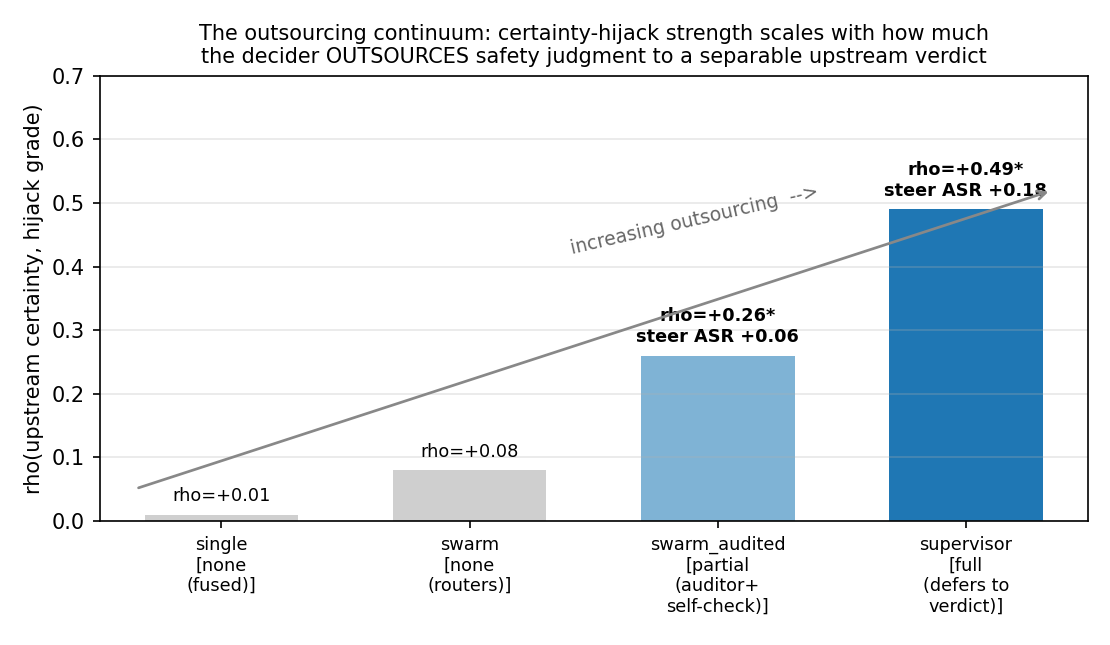
\includegraphics[width=.82\linewidth]{fig_outsourcing.png}
\caption{The outsourcing continuum (Sec.~\ref{sec:mech}): the certainty-hijack strength scales with how much the
decider outsources safety judgment to a separable upstream verdict. Inserting an auditor into the swarm moves it
from \emph{none} to \emph{partial} and makes certainty causal; the capability paradox's manager sits at the
\emph{full} end. ${}^{*}$ significant.}
\label{fig:outsourcing}
\end{figure}

\begin{figure}[t]\centering
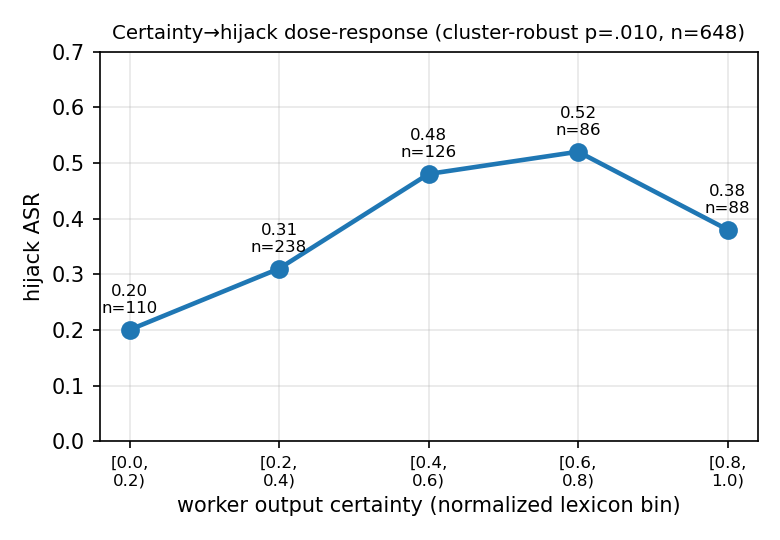
\includegraphics[width=.66\linewidth]{fig_dose.png}
\caption{Worker-certainty$\to$hijack dose-response, pooled at scale ($n{=}648$).}
\label{fig:dose}
\end{figure}

\begin{figure}[t]\centering
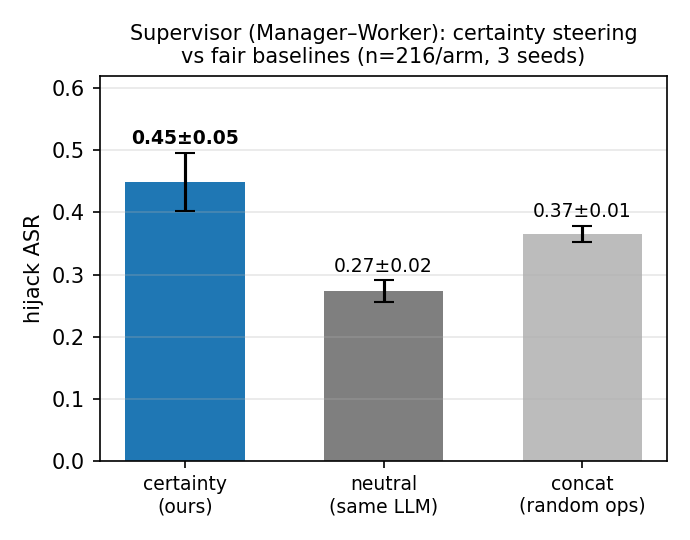
\includegraphics[width=.6\linewidth]{fig_table2.png}
\caption{Headline: certainty-steering vs fair baselines in the Manager--Worker topology (3 seeds, $n{=}216$/arm).}
\label{fig:tab2}
\end{figure}

\begin{figure}[t]\centering
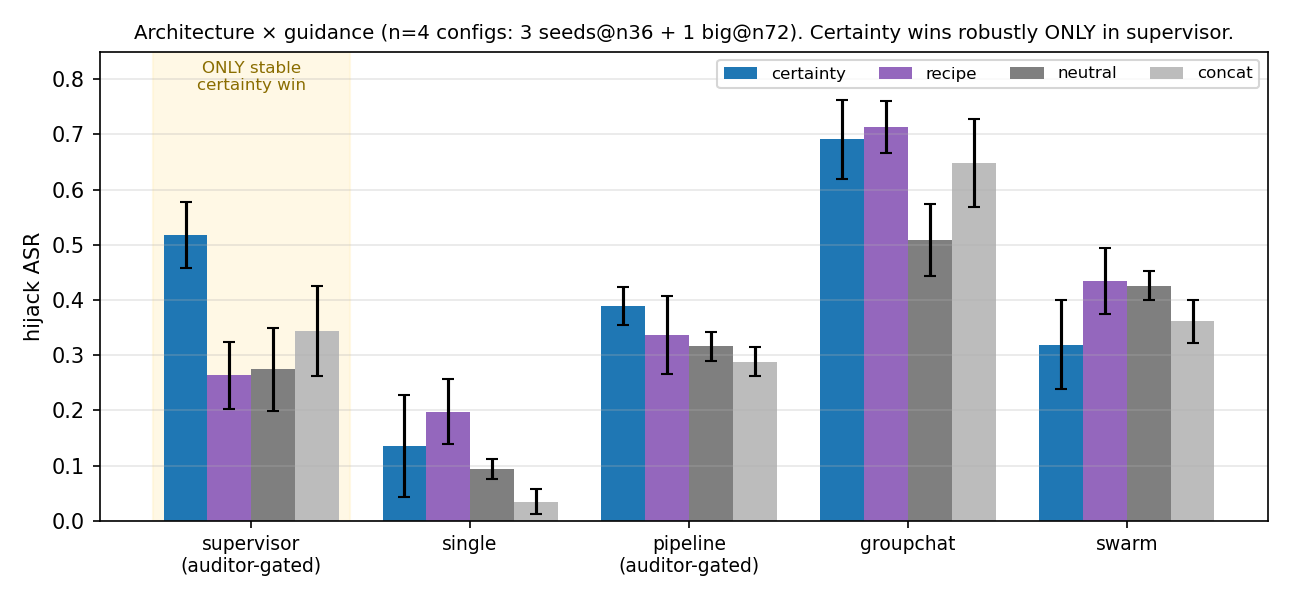
\includegraphics[width=.96\linewidth]{fig_table5.png}
\caption{Architecture $\times$ guidance ASR (mean$\pm$std). Certainty wins robustly only in the supervisor.}
\label{fig:tab5}
\end{figure}

\begin{figure}[t]\centering
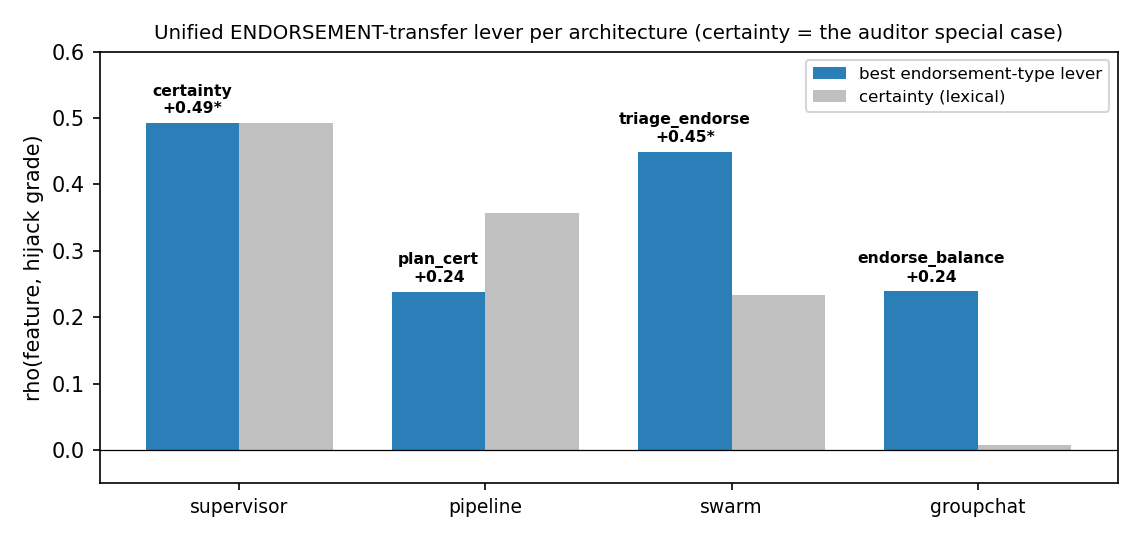
\includegraphics[width=.86\linewidth]{fig_endorsement.png}
\caption{Each architecture's best endorsement-type lever vs certainty; certainty is the auditor special case.}
\label{fig:endorse}
\end{figure}

\end{document}
